\chapter{The title of chapter one}

Lorem ipsum dolor sit amet, consectetur adipiscing elit. Donec non ante sem. Aliquam volutpat nisi erat, quis pharetra nunc lobortis eget. Nam elementum urna mattis, tincidunt eros porttitor, vehicula dui. Integer nisi erat, mattis eget pretium nec, luctus ac neque. Quisque volutpat, dolor nec facilisis pharetra, diam est efficitur ligula, sit amet tincidunt nunc ante at mauris. Integer mattis ultricies dolor, sit amet sagittis nulla facilisis ut. Duis imperdiet ultrices metus, eget fringilla tortor tincidunt non. Nunc condimentum justo at neque consectetur aliquam. Aliquam eu enim sapien. Vivamus sodales nunc ligula, sed sagittis mauris cursus vitae. Etiam sit amet leo sollicitudin, iaculis enim dignissim, aliquet lorem. Aliquam varius euismod risus, sit amet posuere mi pharetra eu. Sed tempor, velit id tristique gravida, elit nunc ultricies tellus, a elementum arcu ante vitae dui. Suspendisse fringilla leo id nisi ultricies, id imperdiet purus tristique. Maecenas non tincidunt risus $x = 1/\alpha$ magna rhoncus neque, id pulvinar odio lorem non turpis \cite{brin2012reprint, russell1995artificial}. Nullam sit amet enim. Suspendisse id velit vitae ligula volutpat condimentum. Aliquam erat volutpat. Sed quis velit. Nulla facilisi. Nulla libero. Vivamus pharetra posuere sapien. Nam consectetuer. Sed aliquam, nunc eget euismod ullamcorper, lectus nunc ullamcorper orci, fermentum bibendum enim nibh eget ipsum. Donec porttitor ligula eu dolor. Maecenas vitae nulla consequat libero cursus venenatis. Nam magna enim, accumsan eu, blandit sed, blandit a, eros \cite{google}.

\section{Section 1}
Quisque facilisis erat a dui. Nam malesuada ornare dolor. Cras gravida, diam sit amet rhoncus ornare, erat elit consectetuer erat, id egestas pede nibh eget odio. Proin tincidunt, velit vel porta elementum, magna diam molestie sapien, non aliquet massa pede eu diam. Aliquam iaculis. Fusce et ipsum et nulla tristique facilisis. Donec eget sem sit amet ligula viverra gravida. Etiam vehicula urna vel turpis. Suspendisse sagittis ante a urna. Morbi a est quis orci consequat rutrum. Nullam egestas feugiat felis.

The epipolar lines $l$ can be computed as follows:

\[l'=Fp, l=F^{T}p'\]

Where $F$ is the fundamental matrix for $(p, p')$, thus $F^{T}$ is the fundamental matrix for $(p',p)$. Integer adipiscing semper ligula. Nunc molestie, nisl sit amet cursus convallis, sapien lectus pretium metus, vitae pretium enim wisi id lectus. Donec vestibulum. Etiam vel nibh. Nulla facilisi. Mauris pharetra. Donec augue. Fusce ultrices, neque id dignissim ultrices, tellus mauris dictum elit, vel lacinia enim metus eu nunc.

\section{Section 2}
Pellentesque vel dui sed orci faucibus iaculis. Suspendisse dictum magna id purus tincidunt rutrum. Nulla congue. Vivamus sit amet lorem posuere dui vulputate ornare. Phasellus mattis sollicitudin ligula. Duis dignissim felis et urna. Integer adipiscing congue metus \ref{fig:combinedneuralnetworks}. Etiam non wisi. Sed accumsan dolor ac augue. Pellentesque eget lectus. Aliquam nec dolor nec tellus ornare venenatis. Nullam blandit placerat sem. Curabitur quis ipsum. Mauris nisl tellus, aliquet eu, suscipit eu, ullamcorper quis, magna. Mauris elementum, pede at sodales vestibulum, nulla tortor congue massa, quis pellentesque odio dui id est. Cras faucibus augue.

\begin{figure}[H]
    \centering
    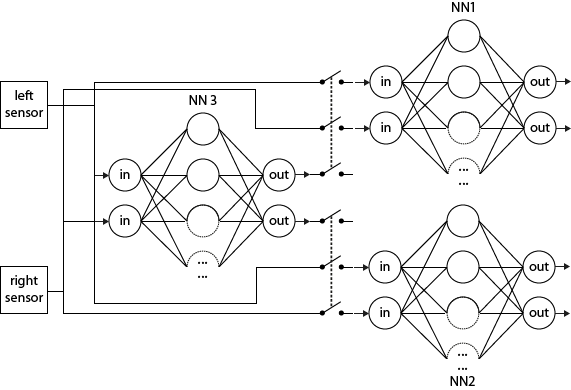
\includegraphics[width=.8\linewidth]{images/figure3.png}
    \caption{Combined neural networks.}\label{fig:combinedneuralnetworks}
\end{figure}

Lorem ipsum dolor sit amet, consectetuer adipiscing elit. Morbi commodo, ipsum sed pharetra gravida, orci magna rhoncus neque, id pulvinar odio lorem non turpis. Nullam sit amet enim. Suspendisse id velit vitae ligula volutpat condimentum. Aliquam erat volutpat. Sed quis velit. Nulla facilisi. Nulla libero. Vivamus pharetra posuere sapien. Nam consectetuer. Sed aliquam, nunc eget euismod ullamcorper, lectus nunc ullamcorper orci, fermentum bibendum enim nibh eget ipsum. Donec porttitor ligula eu dolor. Maecenas vitae nulla consequat libero cursus venenatis. Nam magna enim, accumsan eu, blandit sed, blandit a, eros \ref{tab:results}.

\begin{table}[ht]
	\centering
	\begin{tabular}{ | l | l | l |} \hline
		\textbf{Use encryption} & \textbf{Same keys} & \textbf{Can communicate} \\ \hline
		P1 & - & no \\ \hline
		P1, P2 & no & no \\ \hline
		P1, P2 & yes & yes \\ \hline
	\end{tabular}
	\caption{Two pairs using WEP encryption}
	\label{tab:results}
\end{table}

\section{Section 3}
Quisque facilisis erat a dui. Nam malesuada ornare dolor. Cras gravida, diam sit amet rhoncus ornare, erat elit consectetuer erat, id egestas pede nibh eget odio. Proin tincidunt, velit vel porta elementum, magna diam molestie sapien, non aliquet massa pede eu diam. Aliquam iaculis. Fusce et ipsum et nulla tristique facilisis. Donec eget sem sit amet ligula viverra gravida. Etiam vehicula urna vel turpis. Suspendisse sagittis ante a urna. Morbi a est quis orci consequat rutrum. Nullam egestas feugiat felis. Integer adipiscing semper ligula. Nunc molestie, nisl sit amet cursus convallis, sapien lectus pretium metus, vitae pretium enim wisi id lectus. Donec vestibulum. Etiam vel nibh. Nulla facilisi. Mauris pharetra. Donec augue. Fusce ultrices, neque id dignissim ultrices, tellus mauris dictum elit, vel lacinia enim metus eu nunc.